\documentclass[11pt,a4paper]{article}
\usepackage{zws_companion_style}
\hypersetup{pdftitle={Zero Without Stasis: Organisational Emergence in an Exactly Reversible Signed-Charge-Conserving Block Cellular Automaton},pdfauthor={Chris Bartlett},pdfsubject={Computational study of reversible signed-charge-conserving block dynamics},pdfkeywords={reversible cellular automata, signed charge, finite-time domain formation}}
\graphicspath{{figures/}}
\definecolor{zwsblue}{HTML}{176B87}
\newcommand{\Q}{Q}
\newcommand{\M}{M}
\newcommand{\code}[1]{\texttt{#1}}
\renewcommand{\zwsrunninghead}{Zero Without Stasis}

\begin{document}
\zwstitleblock{Zero Without Stasis}{Organisational Emergence in an Exactly Reversible Signed-Charge-Conserving Block Cellular Automaton}{Chris Bartlett, {\itshape Independent Researcher}. ORCID: \href{https://orcid.org/0009-0001-3323-0131}{0009-0001-3323-0131}\\[1pt]
Companion paper, version 1.49, 13 October 2026. DOI: \href{https://doi.org/10.5281/zenodo.22270456}{10.5281/zenodo.22270456}\\[1pt]
Working paper.\\[1pt]
Companion to \emph{Something is happening: Occurrence Theory}, DOI: \href{https://doi.org/10.5281/zenodo.22875288}{10.5281/zenodo.22875288}.}

\begin{frontnotice}
This is the computational companion to \emph{Something is happening: Occurrence Theory}. It reports one finite formal example, a reversible artificial world whose signed total stays exactly zero while it organises, and grades every claim by the class of evidence behind it. A later intervention test gave a negative result: its endpoint detector also fired on randomly shuffled worlds, so the test cannot show a causal memory effect.
\end{frontnotice}

\section*{Abstract}
We found a simple artificial world in which random material reorganises into large, irregular regions, some rich in material and some nearly empty, while the net signed charge stays exactly zero and every microscopic step can be undone. The result shows how substantial organisation can develop without breaking the global balance or discarding microscopic information; in this model, the timing of that organisation depends strongly on initial occupancy and its form depends on the local reactions. We study a deterministic four-state block cellular automaton whose cells are empty, positive, negative or bound-neutral, driven by a frozen 256-entry local permutation that was selected in an exploratory search and then held fixed throughout the follow-up experiments. Each update conserves the signed charge $Q=N_{+}-N_{-}$ (positive minus negative cells) but not the occupancy $M=N_{+}+N_{-}+N_{\mathrm b}$ (all non-empty cells); the studied worlds start in the global $Q=0$ sector. A $4096\times4096$ localised-patch trajectory developed irregular domains and, after 65,536 forward phases and the corresponding inverse phases, recovered all 16,777,216 cells exactly. Separate $1024\times1024$ homogeneous-random ensembles, 12 seeds per density, exhibited density-sensitive domain formation with high local compositional disorder. No run at initial occupancy 0.16 crossed the fixed geometrical endpoint (a specified growth of connected empty regions, defined in Section~4) by 262,144 phases; at 0.18, 8/12 crossed by 524,288 phases. The Kaplan--Meier median first passage decreased from 495,616 phases at 0.18 to 65,536 at 0.26. Event-centred morphology favoured distributed change rather than a localised droplet front. In the pooled control protocol, a pure-rotation rule and an active sibling conserving both $Q$ and $M$ each gave 0/16 end-of-window strong-domain passes, versus 10/16 for the selected rule; several single reaction-pair removals also suppressed those passes. The contribution is this reproducible, quantitatively controlled finite-time regime, not reversibility or signed balance alone; the data are finite-time and do not establish an equilibrium phase transition.

\textbf{Keywords:} reversible cellular automata; Margolus block automata; signed charge conservation; coarsening; first passage; intervention diagnostics

\begin{sigbox}{Plain-language significance}
Reversible rules do not prevent macroscopic structure, but dramatic pictures alone do not identify a mechanism. This study pairs an exact cell-for-cell reversal test with waiting-time ensembles, density sweeps, arrangement controls, a matched double-conservation sibling, and reaction-pair ablations. The central result is deliberately narrow: one fully specified reversible, signed-charge-conserving automaton produces delayed, large-scale, irregular organisation from random material, and that behaviour is strongly conditioned by density and by the reaction architecture tested. All trajectories remain exactly recoverable in principle, and were shown to be so in the large direct audit.
\end{sigbox}

\section{Introduction}
This paper is the computational companion to \emph{Something is happening} \citep{Bartlett2026ZWS}, which proposes exactly this kind of experiment (its Section 15.3, on \emph{Signed Life}) and states in advance what a simulation can and cannot show for that framework. The present study stands on its own as a finite computational result; the parent paper's metaphysical claims are neither assumed nor tested here. The model is a finite, fixed-lattice realisation of that Signed Life programme; it does not implement the distinct splitting-and-merging refinement conjecture of the parent paper's Sections 2.7 and 15.3, the conjecture that motivated the work. Experiment and preregistration dates are documented in the archived records cited in Section~9, on code and data availability.

Reversible cellular automata and lattice gases have long supplied constructive examples of local invertibility, conservation, and emergent statistical behaviour \citep{FredkinToffoli1982,Margolus1984,Vichniac1984,ToffoliMargolus1987,ToffoliMargolus1990}. Conservative lattice gases recover transport and hydrodynamic phenomena \citep{HPP1973,FrischHasslacherPomeau1986,RothmanZaleski1994,BoonEtAl1996}; reversible Ising and Q2R models display relaxation, long cycles, and phase-like macroscopic behaviour \citep{Creutz1986,Takesue1987,UrbinaRica2016,Urbina2020,MontalvaMedelRicaUrbina2020}; and reversible aggregation shows that invertible local dynamics can support cluster growth \citep{DSouzaMargolus1999}. More recent one-dimensional reversible automata with vacancies and two particle species provide close alphabet, reaction, and conserved-charge precedents \citep{MedenjakPopkovProsen2019,KlobasProsen2022}, while reactive lattice-gas automata provide established examples of waves and pattern formation \citep{KapralLawniczakMasiar1991}. We therefore make no claim that reversibility plus organisation, multi-species reversible dynamics, or reaction-driven patterning is new in itself.

The narrower question is what can be established for a four-state signed system in which one additive quantity is exact while total occupancy can change. The distinction matters. A rule may conserve
\begin{equation}
Q=N_{+}-N_{-},
\end{equation}
without conserving
\begin{equation}
M=N_{+}+N_{-}+N_{\mathrm b}.
\end{equation}
Writing ``$Q=0$'' describes the global sector of the runs, not a second local conservation law and not an empty world. This paper asks whether a frozen rule in that architecture, one selected in the exploratory search and then held fixed, never re-tuned, through all follow-up experiments, reproducibly forms large irregular domains, how density and waiting time condition the outcome, and which nearby rule controls retain or suppress that behaviour.

Our terminology is descriptive. ``Coarsening-like'' refers to growth of long-wave structure and connected regions over the observed finite lattice and time window. ``Strong-domain'' refers to a fixed operational endpoint. Neither term asserts equilibrium phase separation, a critical point, a free-energy description, or a universality class \citep{HohenbergHalperin1977,Bray1994}.

\section{Model and exact audits}
In plain terms, the world is a square grid of cells wrapped into a torus. Every cell is in one of four states: empty, positive, negative, or bound-neutral. Time advances in phases. In each phase the grid is cut into $2\times2$ blocks, with the cut shifted diagonally by one cell on alternate phases so that no block boundary is permanent, and every block is replaced by looking up its four-cell pattern in a fixed table of 256 entries. The table is a permutation of those 256 patterns, so each phase can be undone exactly by looking up the inverse table. Two counts matter throughout. The signed charge $Q$, positive cells minus negative cells, is unchanged by every table entry: it is a hard law of this world, not a quantity corrected afterwards. The occupancy $M$, the number of non-empty cells, is free: some entries create or remove a balanced positive--negative pair, so material can be made and unmade while $Q$ stays put. That freedom is what the matched controls of Section~5.4 probe.

\subsection{Four-state partitioned dynamics}
Each square-lattice cell takes a value in $\{0,+,-,\mathrm b\}$: empty, positive excitation, negative excitation, or bound-neutral excitation. Alternating $2\times2$ Margolus partitions tile the periodic lattice. The four input symbols of each block are packed into one of 256 block states; a 256-entry permutation maps that block state to an output state. Applying the inverse permutation in reverse phase order recovers the predecessor exactly. The selected rule, called the winner throughout, has a raw unsigned-byte table with SHA-256
\begin{center}
\code{d1fe99b5735d8e9be032347de2727dc5c52a7848df200ca26f67f28c8c1bc41c}.
\end{center}
All 256 local cases were exhaustively audited. For every block input, the permutation is one-to-one and preserves the block contribution to $Q$. The winner does not preserve the block contribution to $M$; bound/unbound and occupied/empty reaction channels allow occupancy to change while signed balance remains exact. The construction starts from clockwise block rotation and exchanges 12 reversible pairs of outputs, so 24 of the 256 input blocks differ from pure rotation. Figure~\ref{fig:rule-worked} shows the alternating partition and two entries from the archived table, including an actual reaction in which a balanced positive--negative pair is added while $Q$ is unchanged.

An elementary count says how much room exact balance leaves. Each cell contributes $+1$, $-1$ or $0$ to $Q$, and two of the four symbols, empty and bound-neutral, contribute $0$. The number of configurations of $n$ cells with $Q=0$ is therefore the constant term of $(z^{-1}+2+z)^n=z^{-n}(1+z)^{2n}$, which is the central binomial coefficient $\binom{2n}{n}$ \citep[Chapter~5]{GrahamKnuthPatashnik1994}. For a single $2\times2$ block this is 70 of the 256 inputs; for a lattice of $N$ cells it is $\binom{2N}{N}$, and because the complete state includes the partition phase, the space of complete neutral states holds two copies of each configuration, one per phase. This is a count of allowed configurations, not a measured orbit length, an equilibrium measure or evidence that the winner reaches every neutral configuration: it quantifies the freedom compatible with zero charge without explaining the observed organisation.

\subsection{Large exact reversal}
The audited $4096\times4096$ trajectory began with a random central square spanning 45\% of each lattice dimension, the rest of the lattice empty. Within the patch the target state fractions were 12\% positive, 12\% negative and 8\% bound-neutral, with exact positive--negative balance. It was advanced for 65,536 partition phases and then evolved backwards with the exact inverse schedule. The recovered lattice matched its initial state at all 16,777,216 cells. Global $Q$ remained zero throughout; $M$ changed substantially. This is an implementation and coexistence audit, not a claim that reversibility itself is novel.


\begin{figure}[p]
\centering
{\Large\bfseries Reversible dynamics, changing structure\par}
\vspace{0.15em}
{\small Zero net signed charge throughout; occupancy is free to change\par}
\vspace{0.55em}
\begin{minipage}[t]{0.437\linewidth}
\textbf{A\quad Initial localised random patch}\\[-0.1em]
{\small Global $Q=0$; $M=1{,}085{,}747$}\par\vspace{0.2em}
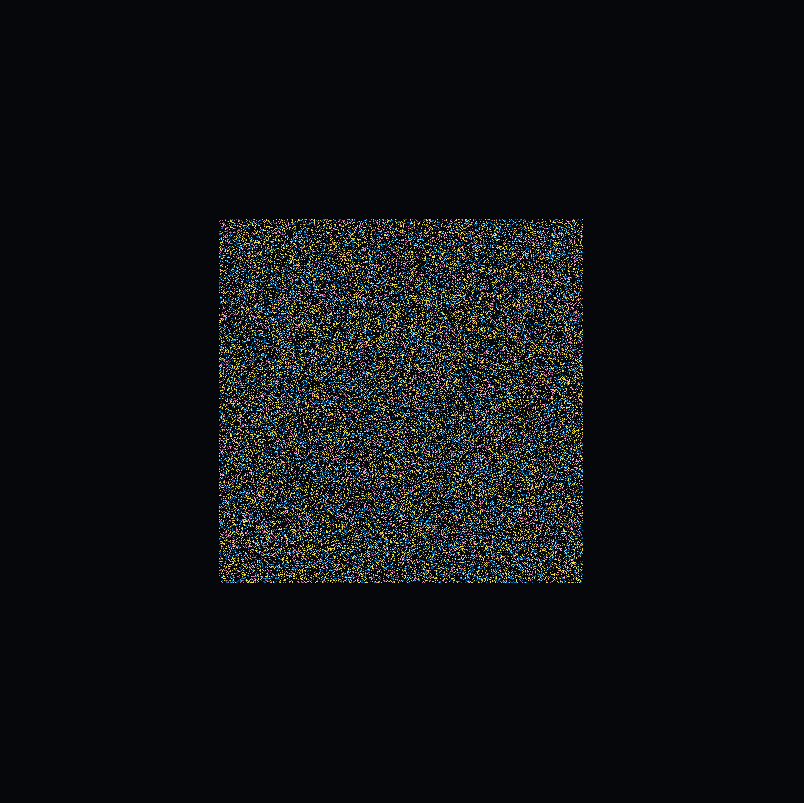
\includegraphics[width=\linewidth]{figure_assets/hero_v024/panel_A.png}\\[-0.1em]
{\small $4096\times4096$ cells; phase 0}
\end{minipage}\hfill
\begin{minipage}[t]{0.437\linewidth}
\textbf{B\quad Same world after 20,480 phases}\\[-0.1em]
{\small Global $Q=0$; $M=1{,}624{,}064$}\par\vspace{0.2em}
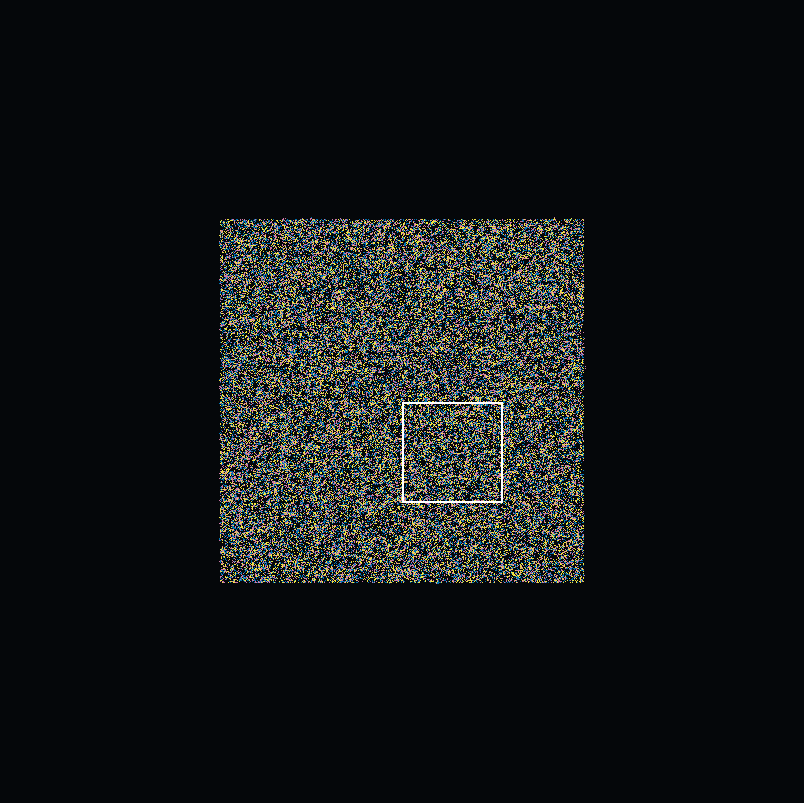
\includegraphics[width=\linewidth]{figure_assets/hero_v024/panel_B.png}\\[-0.1em]
{\small $4096\times4096$ cells; phase 20,480}
\end{minipage}
\vspace{0.45em}

\begin{minipage}[t]{0.437\linewidth}
\textbf{C\quad Enlarged region of B}\\[-0.1em]
{\small $512\times512$ crop at $x=2048$, $y=2048$}\par\vspace{0.2em}

\includegraphics[width=\linewidth]{figure_assets/hero_v024/panel_C.png}\\[-0.1em]
{\small Whole-world $Q=0$; $M=1{,}624{,}064$}
\end{minipage}\hfill
\begin{minipage}[t]{0.437\linewidth}
\textbf{D\quad Initial state, recovered exactly}\\[-0.1em]
{\small Global $Q=0$; $M=1{,}085{,}747$}\par\vspace{0.2em}
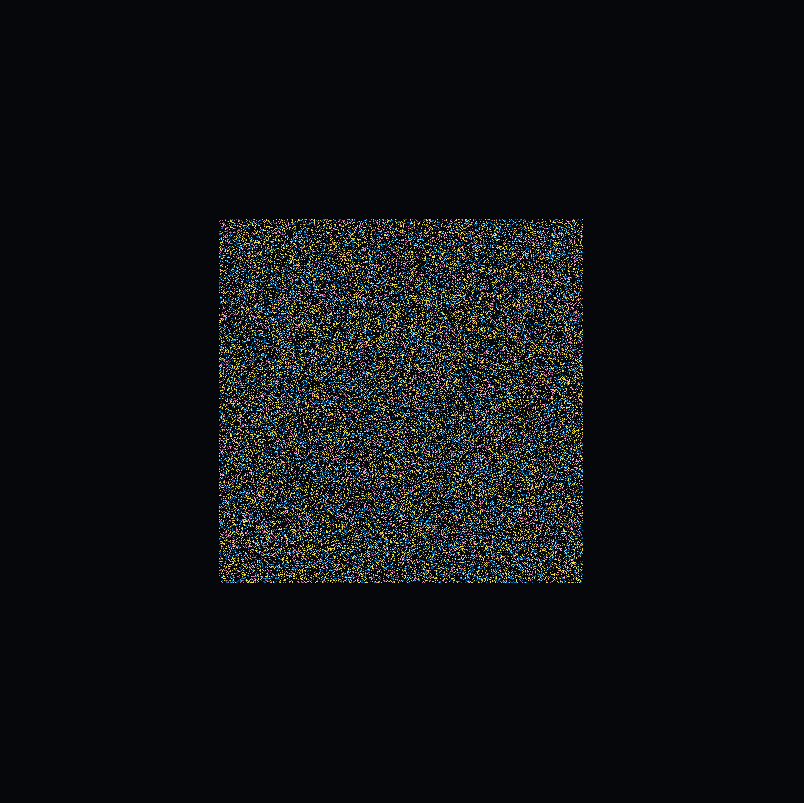
\includegraphics[width=\linewidth]{figure_assets/hero_v024/panel_D.png}\\[-0.1em]
{\small 65,536 forward + 65,536 inverse phases}
\end{minipage}
\vspace{0.45em}

{\small
\colorbox[HTML]{05070A}{\rule{0pt}{1.1ex}\hspace{1.25ex}}\,empty\qquad
\colorbox[HTML]{F0E442}{\rule{0pt}{1.1ex}\hspace{1.25ex}}\,positive\qquad
\colorbox[HTML]{0072B2}{\rule{0pt}{1.1ex}\hspace{1.25ex}}\,negative\qquad
\colorbox[HTML]{CC79A7}{\rule{0pt}{1.1ex}\hspace{1.25ex}}\,bound-neutral\par}
\vspace{0.2em}
{\small\bfseries Exact reversal: zero mismatches across all 16,777,216 cells.\par}
\caption{\textbf{Reversible dynamics, changing structure.} A and B show the world at phases 0 and 20,480; C enlarges the boxed $512\times512$ region of B, where the reorganisation can be seen. D is the phase-0 state, recovered exactly by the separate reversal audit. One localised-patch trajectory.}
\label{fig:hero}
\end{figure}

\section{Discovery, selection, and confirmation}
\subsection{A small, explicitly selective search}
The winner was search-selected, not sampled blindly. The original discovery run was a small-scale exploratory search, a ``smoke'' run in the software's terms; it evaluated 14 unique rules over 16~replicate evaluations in a reactive-rotation construction family. Its declared heuristic rewarded intermediate bands of activity, reaction density, state and block entropy, spatial and temporal mutual information, recurrence, perturbation distance, and patch repetition, with a dynamics gate and a hard charge-preservation gate. The behaviour reported below therefore cannot be described as wholly unselected.



\begin{figure}[!b]
\centering
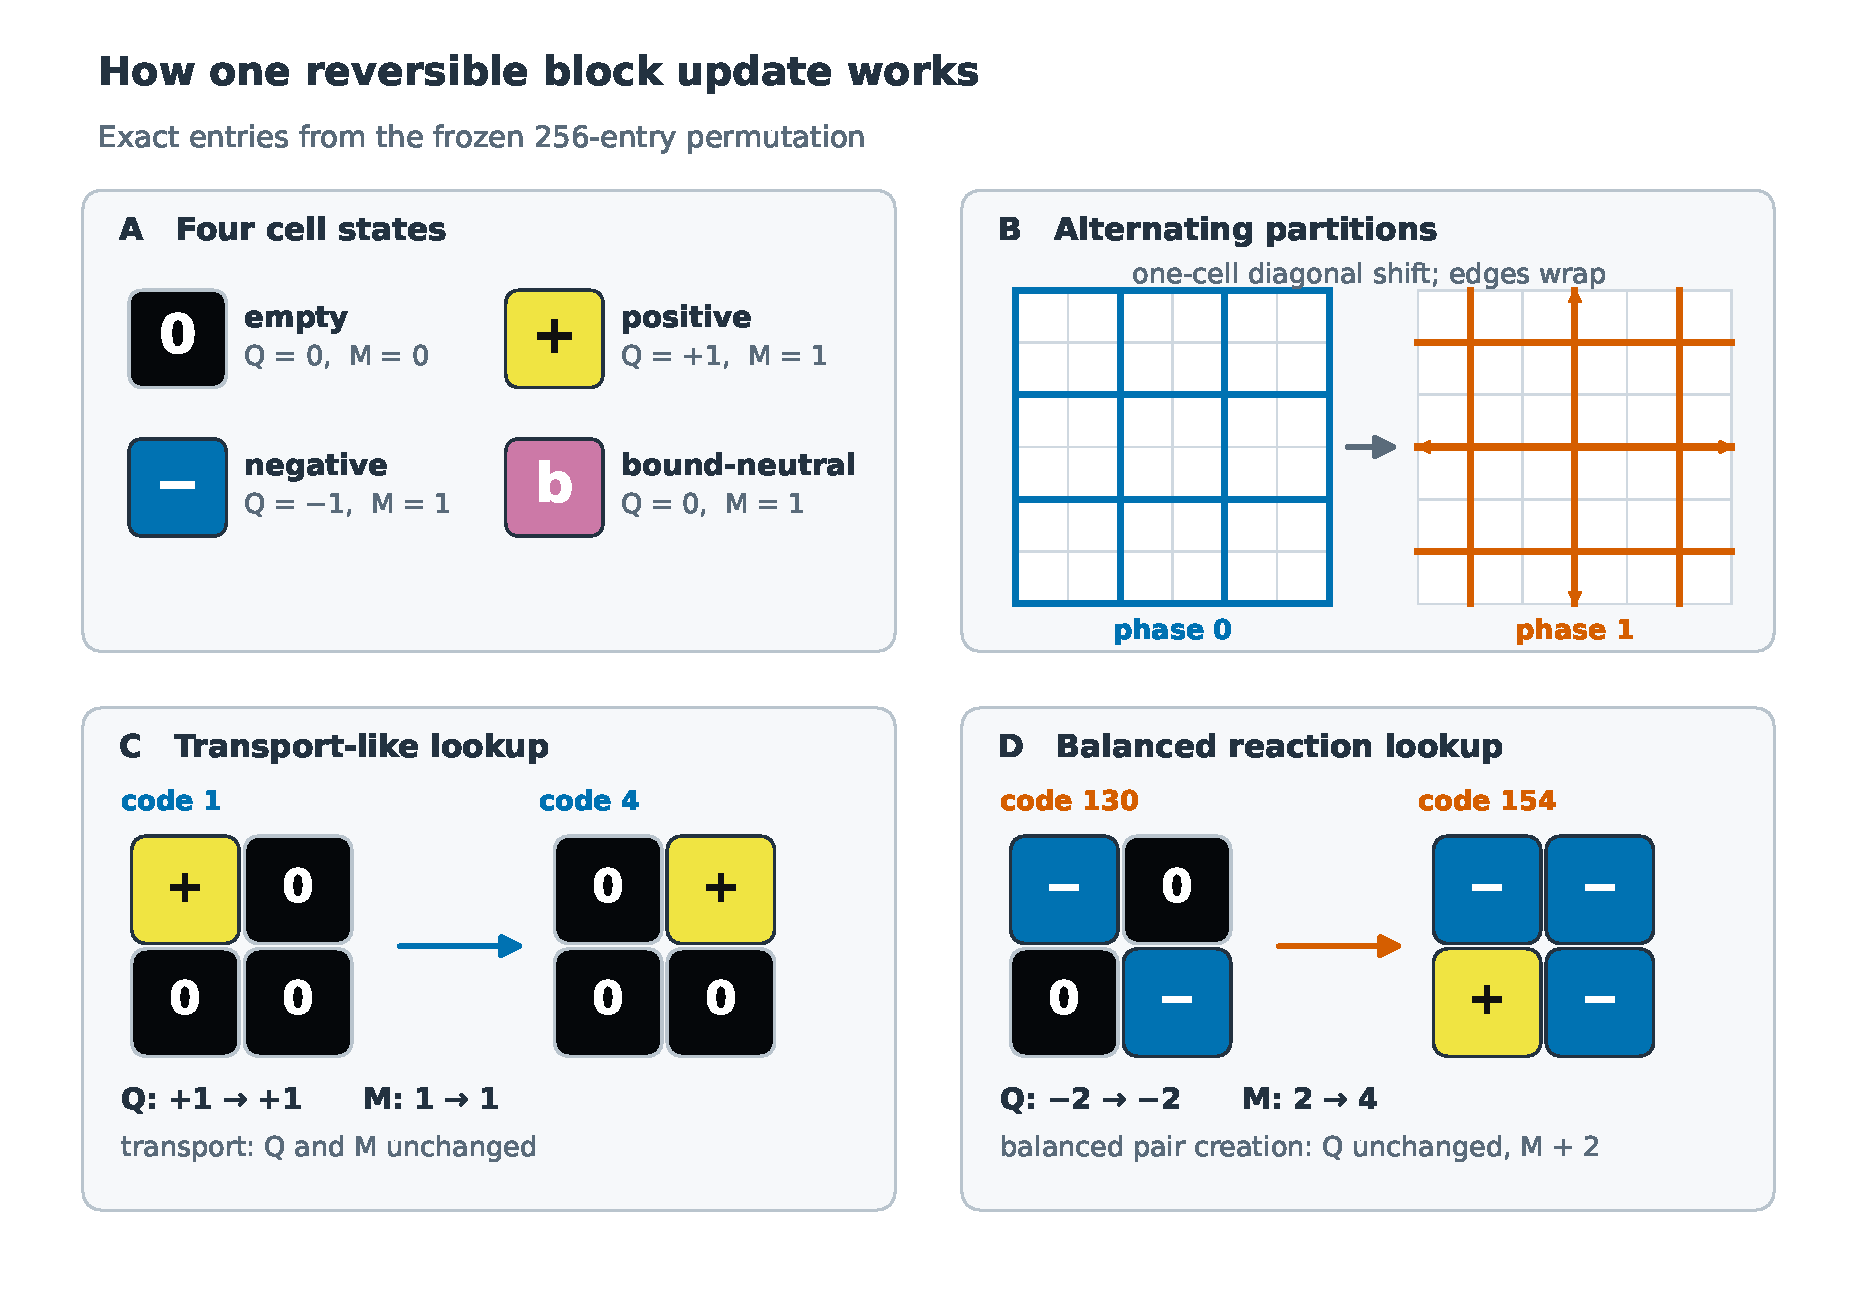
\includegraphics[scale=0.5]{COMPANION_V135_FIGURE_02_HOW_THE_RULE_WORKS.pdf}
\caption{\textbf{One reversible block update.} A: cell states and their charge $Q$ and occupancy $M$. B: alternating $2\times2$ partitions. C and D: exact table entries $1\mapsto4$ and $130\mapsto154$; cell order is top-left, top-right, bottom-left, bottom-right.}
\label{fig:rule-worked}
\end{figure}

The discovery score did \emph{not} use the later $4096^2$ reversal result, the density first-passage curves, the event morphology, the arrangement controls, the double-conservation sibling, the reaction-pair ablations, the prevalence screen, or the later classifier diagnostics. Those were frozen and run as follow-up measurements. The exact search provenance and metric weights are retained with the release.

\subsection{Separation of evidence classes}
We use four labels. \emph{Discovery} denotes the tiny search and exploratory smoke run. \emph{Confirmation} denotes frozen winner repeats and the large exact reversal. \emph{Mechanism constraints} denote preregistered density, geometry, sibling, and ablation comparisons. \emph{Diagnostics} denote analyses that reveal a limitation in the assay and so cannot answer the causal question they were built for. Results below state their class rather than pooling them as if they were exchangeable.

The later prevalence screen found 19 strong-domain rules among 256 independently generated charge-preserving candidates (7.4219\%; Wilson 95\% interval 4.8026--11.3001\%). This shows that the operational regime is not unique to one table within the sampled generator, but it neither erases the original selection nor estimates prevalence in all $256!$ block permutations.

\section{Measurements}
The strong-domain endpoint of the v0.3 and v0.3.1 campaigns is a geometrical, trajectory-prefix classifier; it does \emph{not} include a spectral-growth threshold. In words, the flag fires once the finite (non-wrapping) empty regions have grown, at some past sample, to at least four times their initial characteristic scale; still stand at least twice that initial scale at the current sample; the largest such region at that peak sample covers at least 0.1\% of the lattice; and the global charge has never changed. Formally, let $L_j$ be the measured characteristic scale of finite empty components at sampled phase $t_j$, let $r_j=L_j/\max(L_0,1)$, and let $j^*$ be the first index attaining the largest $r_j$ in the prefix through $t_k$. Writing $f_j$ for the lattice fraction in the largest finite empty component, the implemented flag is
\begin{equation}
 C_k=\mathbf{1}\!\left[
 r_{j^*}\geq4,\quad r_k\geq2,\quad f_{j^*}\geq0.001,
 \quad Q_j=Q_0\ \hbox{for all }j\leq k\right].
 \label{eq:endpoint}
\end{equation}
Here $\mathbf{1}[\cdot]$ equals 1 when every listed condition holds and 0 otherwise. A prefix requires at least two snapshots. Spectral power, interface density, anisotropy and spatial mutual information are \emph{separate measurements}, not additional gates in Eq.~\ref{eq:endpoint}. This distinction is essential for understanding the shuffled-state false positives described in Section~7, on the failed shuffling test.

For the v0.3.1 first-passage study, $T_{\rm hit}$ is the first sampled phase with $C_k=1$. The separate persistent endpoint, $T_{\rm persistent}$, is the first sample at which three consecutive flags are true. Samples are 2,048 phases apart. A transient first hit need not be the persistent hit. Runs that had not crossed by the end of their follow-up (right-censored runs) are kept as censored rather than assigned artificial event times, and a Kaplan--Meier median is reported only when the ensemble actually reached it \citep{KaplanMeier1958,RoystonParmar2013}. Earlier campaigns used related but distinct frozen endpoints; the Supplement states their differences rather than treating all reported pass counts as interchangeable.

All quantitative claims refer to the stored sizes, seeds, phase horizons, and frozen thresholds. The endpoint is useful for comparing these runs but is not a natural law. Exact local-state images are rendered with nearest-neighbour sampling. Reported ``reaction density'' is the fraction of the blocks updated in a phase whose table entry changes the block's multiset of cell states, a reaction entry rather than a rearrangement; it is not a chemical rate constant.

\section{Results}
\subsection{Large-scale order with local compositional disorder}
The localised-patch studies and the later whole-torus homogeneous-random studies both showed broad material-rich regions separated by near-empty regions, under their respective preparation and density conditions. The numerical composition result here comes from the four $4096\times4096$ localised-patch confirmation runs. The dense interior is the high-local-density band, excluding a margin around the dense/sparse interface; its median occupancy at the final stored snapshot of each run was 0.572989, with positive, negative and bound-neutral fractions 0.192542, 0.192535 and 0.187912. Normalised four-state compositional entropy was 0.946343. High single-site diversity is not itself proof of spatial randomness; the images and separately recorded spectral diagnostics support the description of irregular, non-crystalline morphology.

Across those four localised-patch confirmation runs, the transient domain-scale peak ranged from 72.66 to 136.11 times its initial value (median 98.4459), while the final recorded scale remained 15.77 to 16.33 times its initial value (median 16.1118). The effect is large but non-monotone. The preregistered sustained late-time coarsening criterion was not met at this scale; that criterion is a separate, stricter test, which also required continued growth of the empty-domain scale through the late half of the run (Supplement, Section~5.3, on the earlier frozen endpoints). The large transient morphology does not vindicate that stronger hypothesis.

\begin{figure}[!b]
\centering
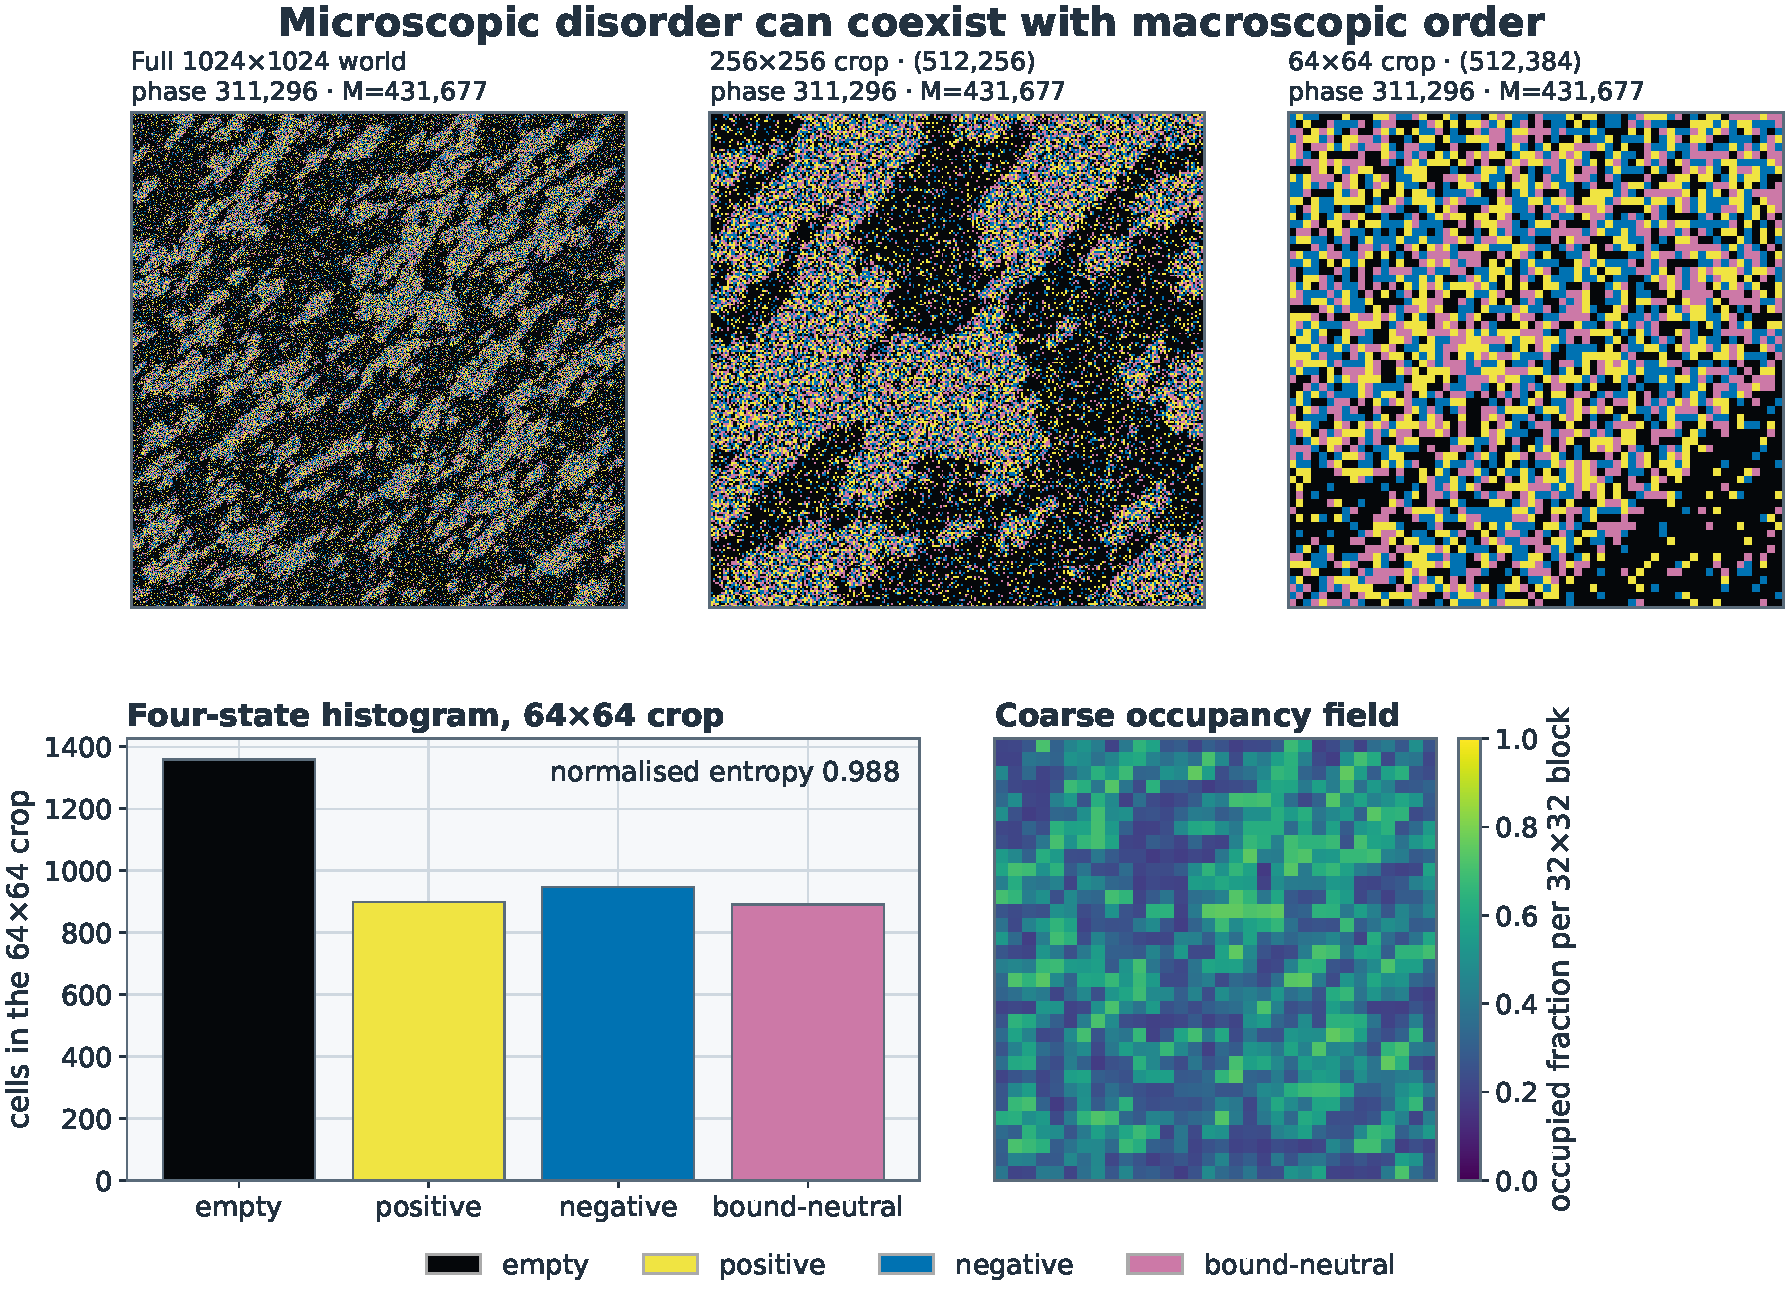
\includegraphics[scale=0.5]{FIGURE_06_MICRO_DISORDER_MACRO_ORDER_V135.pdf}
\caption{\textbf{Microscopic disorder, macroscopic order.} Top: one untouched homogeneous-start world (initial occupancy 0.20, seed 6203), with two nested crops. Bottom: the $64\times64$ crop's four-state histogram and coarse occupancy averaged over $32\times32$ blocks.}
\label{fig:micro-macro}
\end{figure}

\subsection{Density controls waiting time}
The first-passage cohort comprised homogeneous-random $1024\times1024$ worlds. At an initial occupancy of 0.16, none of 12 runs reached the endpoint within 262,144 phases. At 0.18, 8/12 reached it in the extended 524,288-phase campaign, with median first passage 495,616 phases. All 12 replicates reached it at each tested density from 0.20 through 0.26; median first passage fell from 321,536 phases at 0.20 to 65,536 at 0.26 (Table~\ref{tab:density}). Across 0.18 to 0.26 the medians lie close to a straight line on a logarithmic scale: each percentage point removed from the starting occupancy lengthens the median wait by a factor of about 1.3 (an unweighted least-squares fit of log median phase against initial occupancy, six points, $R^2=0.995$; descriptive, not a law). Within the v0.3/v0.3.1 endpoint, longer observation admitted events at occupancies whose runs rarely crossed at shorter horizons. The earlier onset figure of approximately 27.5\% came from a related but different frozen classifier, and is not a numerically interchangeable threshold estimate. The defensible result is strong finite-time density dependence, not an equilibrium critical density.

\begin{table}[tb]
\centering
\caption{Homogeneous $1024^2$ first-passage cohort, with actual follow-up horizons.}
\label{tab:density}
\begin{tabular}{@{}rrrr@{}}
\toprule
Initial occupancy & Events / 12 & KM median (phases) & Follow-up horizon (phases) \\
\midrule
0.16 & 0  & not reached & 262,144 \\
0.18 & 8  & 495,616 & 524,288 \\
0.20 & 12 & 321,536 & 262,144 / 524,288$^{a}$ \\
0.22 & 12 & 206,848 & 262,144 \\
0.24 & 12 & 108,544 & 262,144 \\
0.25 & 12 & 83,968  & 262,144 \\
0.26 & 12 & 65,536  & 262,144 \\
\bottomrule
\multicolumn{4}{@{}p{0.94\linewidth}@{}}{\footnotesize Homogeneous $1024^2$ worlds; Kaplan--Meier median is the first sample at which the estimated survival is at most $1/2$, not the median of observed events alone. $^{a}$At occupancy 0.20, two already-transformed runs retained their 262,144-phase record and ten censored trajectories continued to 524,288. Four of the 0.18 trajectories remained right-censored. Recorded horizons, not an imputed common duration, are shown.}
\end{tabular}

\end{table}

\begin{figure}[!b]
\centering
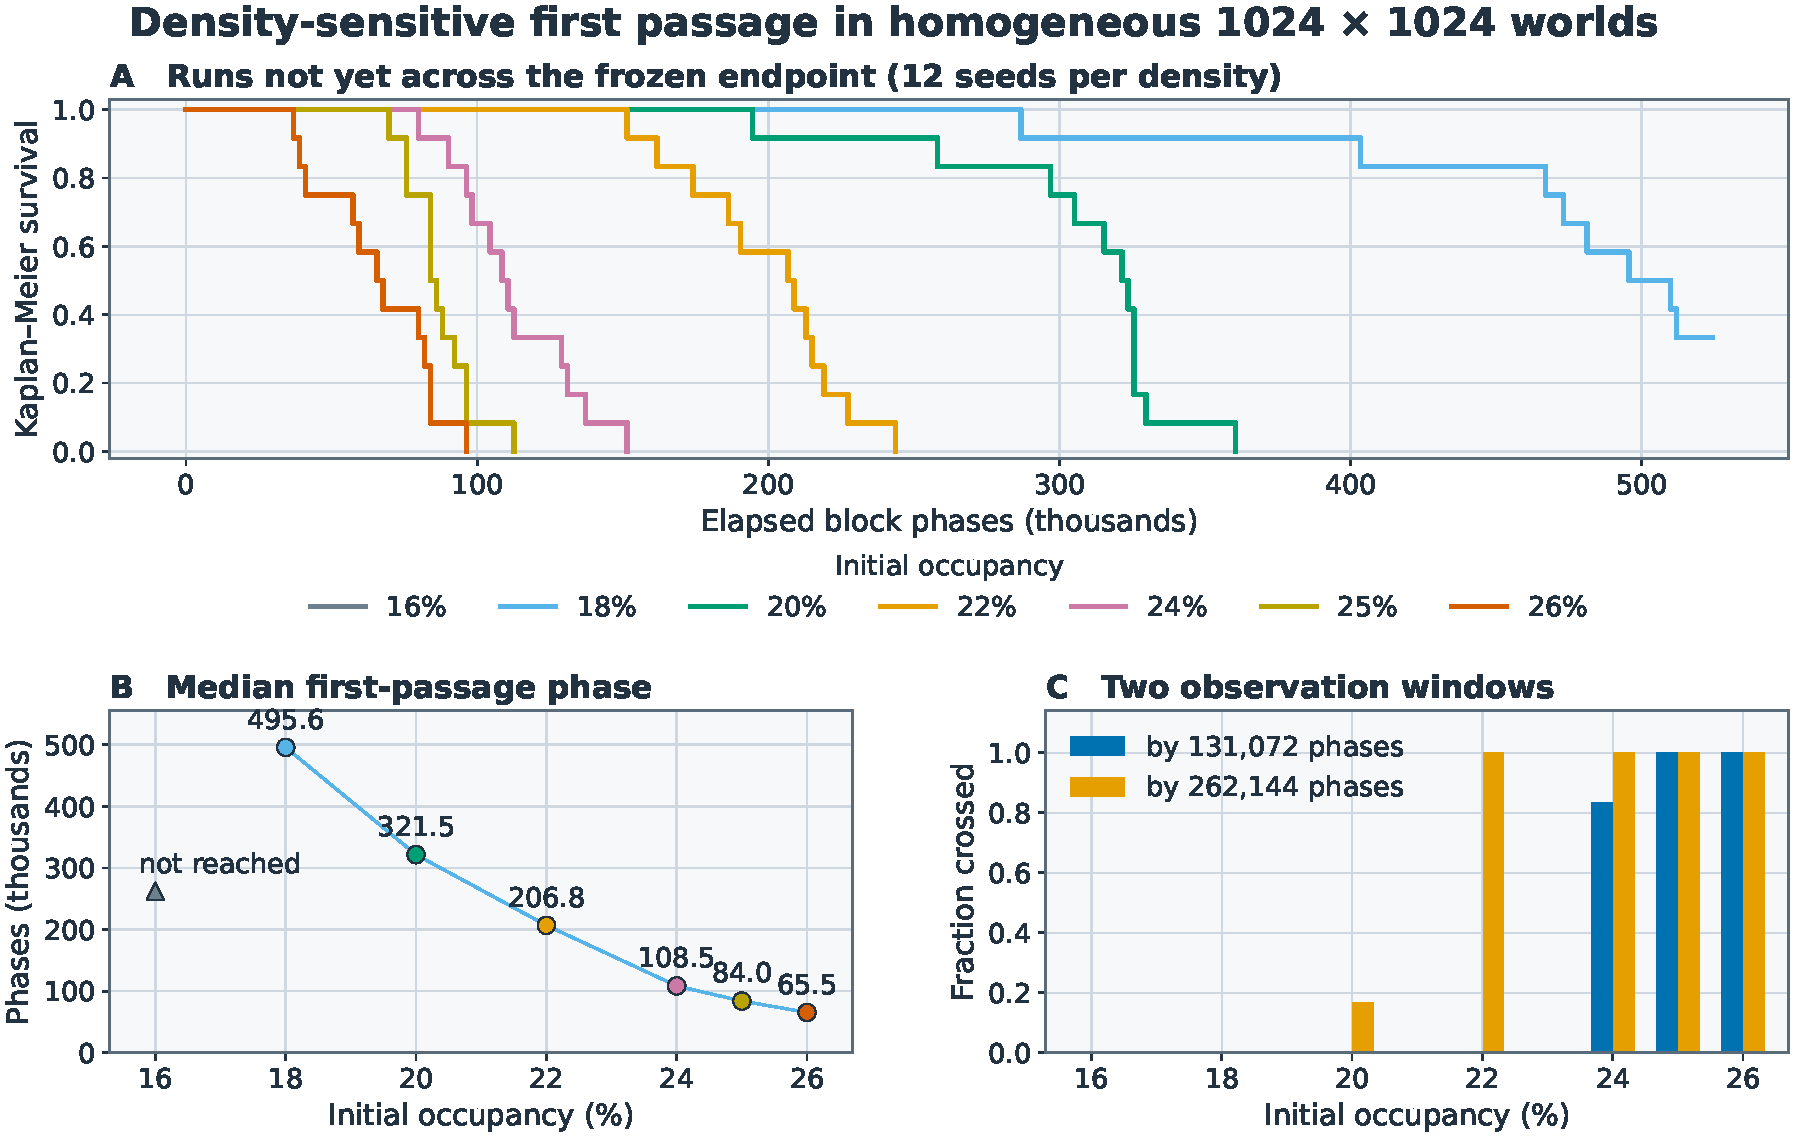
\includegraphics[scale=0.5]{COMPANION_V135_FIGURE_03_DENSITY_FIRST_PASSAGE.pdf}
\caption{\textbf{Density and waiting time.} A: Kaplan--Meier survival, 12 seeds per initial occupancy. B: Kaplan--Meier median first-passage phase; the 0.16 ensemble remains uncrossed at 262,144 phases. C: fractions crossed by 131,072 and 262,144 phases.}
\label{fig:density}
\end{figure}

\subsection{Distributed events and the prepared-geometry comparison}
Each endpoint crossing was examined in a frozen window of the samples leading up to it and labelled by where the change happened. A crossing is \emph{localised} if at least half of the sites whose occupancy changed lay inside one crop covering a sixteenth of the lattice, placed once where the change across the window was densest and then held fixed (the signature a single growing nucleus would leave). It is \emph{distributed} if that crop held no more than an eighth of the changed sites while the finite-empty scale grew in at least half of the pre-hit intervals, and \emph{unresolved} otherwise. Two further preregistered labels, merger and reconnection, matched no event. The pool is the 91 first hits observed in the v0.3.1 study, 68 from the primary $1024^2$ cohort and 23 from the $512^2$ area-scaling cohort. The labels classified 67 transitions as distributed, 24 as unresolved, and none as localised droplet-front events. Under a simple local Poisson picture, in which independent nucleation events occur at a fixed rate per cell and the delay from nucleation to detection is negligible, the event rate per phase of exposure divided by the number of cells would be the same on the matched $512^2$ and $1024^2$ lattices; instead the smaller lattice showed roughly four times that per-cell rate at every matched density, so that picture was not supported. These finite-window observations constrain a localised-front interpretation without excluding every nucleation description or establishing an asymptotic rate law.

Prepared starts place the same occupied inventory in a single compact disc (a droplet) or a single full-height band (a slab), at a set internal density with the rest of the torus empty. They produced 0/48 endpoint crossings by 262,144 phases, versus 19/24 for matched homogeneous starts, while their imposed occupied structures persisted or grew. Crucially, Eq.~\ref{eq:endpoint} measures finite empty-component growth relative to each trajectory's own initial finite-empty-domain scale; it is not an occupied-seed survival test. Preparing a large occupied shape changes both the starting geometry and the normalisation baseline, relative to random soup. The pass-count contrast is not a shared absolute test of whether a large structure forms or survives, and it cannot by itself show that seeded organisation fails or that compact seeds inhibit the phenomenon. The direct persistence measurements and the relative-growth endpoint must be read separately.

\subsection{Conservation and reaction controls constrain the mechanism}
The closest tested reactive sibling is a variant of the winner, altered so that every block update conserves $M$ as well as $Q$ while keeping non-zero reactions; among the candidates tested it is the nearest such variant, not a proven minimum. It remained dynamically active (the median across runs of the mean reaction density was 0.01160, versus 0.01234 for the winner) but produced 0/8 strong-domain outcomes in the focused $1024^2$ screen (8 replicates) and 0/16 end-of-window strong-domain passes in the pooled $512^2$ balanced protocol (16 replicates); the winner produced 8/8 and 10/16 respectively. A pure-rotation control also produced 0/16. Thus inactivity alone does not explain the sibling result, and transport alone is insufficient under this protocol.

The effects of single reaction-pair removals were heterogeneous. Six of twelve tested pair removals produced no end-of-window pass in any of their 16 replicates; the other removals left between 2 and 7 end-of-window passes. These pooled counts are taken at the end of the observation window and are not first-passage counts: a run can cross the endpoint and later fall back below the final scale-ratio threshold, which happened to one run in each of two ablations. From these data, the architecture is therefore distributed across several channels rather than reducible to one uniquely necessary pair. Table~\ref{tab:controls} and Figure~\ref{fig:controls} report the full pooled comparison.

An elementary signed toy control makes the same point about $Q$ without any dynamics. Assign the signs $\pm1$ uniformly at random to $N$ sites, with $N$ even, subject only to exact global neutrality, $\sum_i s_i=0$. Squaring that constraint gives $N+\sum_{i\neq j}s_is_j=0$. The ensemble treats every pair of sites alike, so for any two distinct sites $\langle s_is_j\rangle=-1/(N-1)$, whatever their separation. Global sign balance in this ensemble fixes only that separation-independent two-point correlation; it imposes no distance-dependent structure of its own. Any distance-dependent organisation in the four-state dynamics is therefore not explained by the constraint $Q=0$ alone.

\begin{table}[tb]
\centering
\caption{Matched controls and single-pair ablations: end-of-window strong-domain passes under the pooled $512^2$ protocol, 16 replicates each.}
\label{tab:controls}
\resizebox{\linewidth}{!}{\begin{tabular}{@{}lrrl@{}}
\toprule
Condition & Strong-domain passes & Trials & Interpretation at tested protocol \\
\midrule
Frozen winner (exact $Q$) & 10 & 16 & reference \\
Reactive exact-$Q{+}M$ sibling & 0 & 16 & active, no winner regime \\
Pure rotation & 0 & 16 & transport-only negative control \\
Ablations 01, 11 & 7 each & 16 each & partial retention \\
Ablation 05 & 6 & 16 & partial retention \\
Ablations 08, 09 & 3 each & 16 each & strong attenuation \\
Ablation 06 & 2 & 16 & strong attenuation \\
Ablations 00, 02, 03, 04, 07, 10 & 0 each & 16 each & suppression \\
\bottomrule
\end{tabular}
}
\end{table}

\begin{figure}[p]
\centering
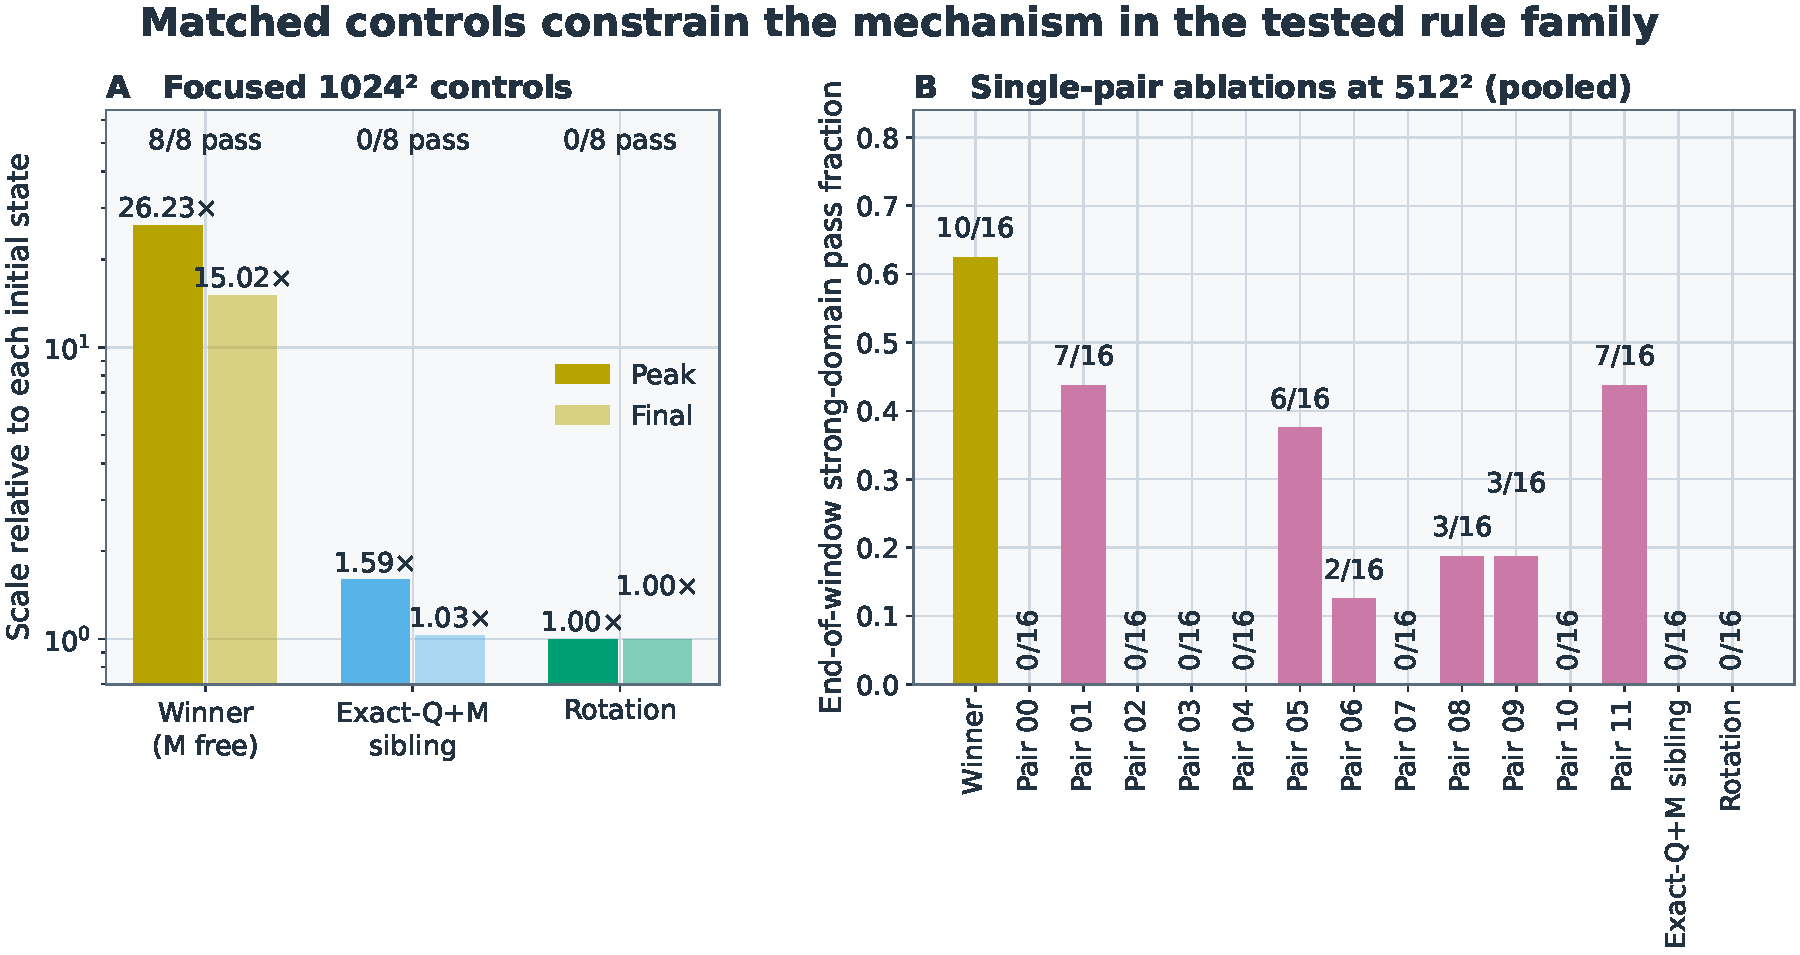
\includegraphics[scale=0.5]{COMPANION_V135_FIGURE_04_CONTROLS_AND_ABLATIONS.pdf}
\caption{\textbf{Matched controls and reaction-pair removals.} A: medians across eight replicates of peak and final finite empty-domain scale relative to each run's initial scale; labels give strong-domain outcomes. B: end-of-window pass fractions in a separate $512^2$ protocol, 16 replicates per condition; each pair label identifies one reaction-pair removal.}
\label{fig:controls}
\end{figure}

\begin{figure}[p]
\centering
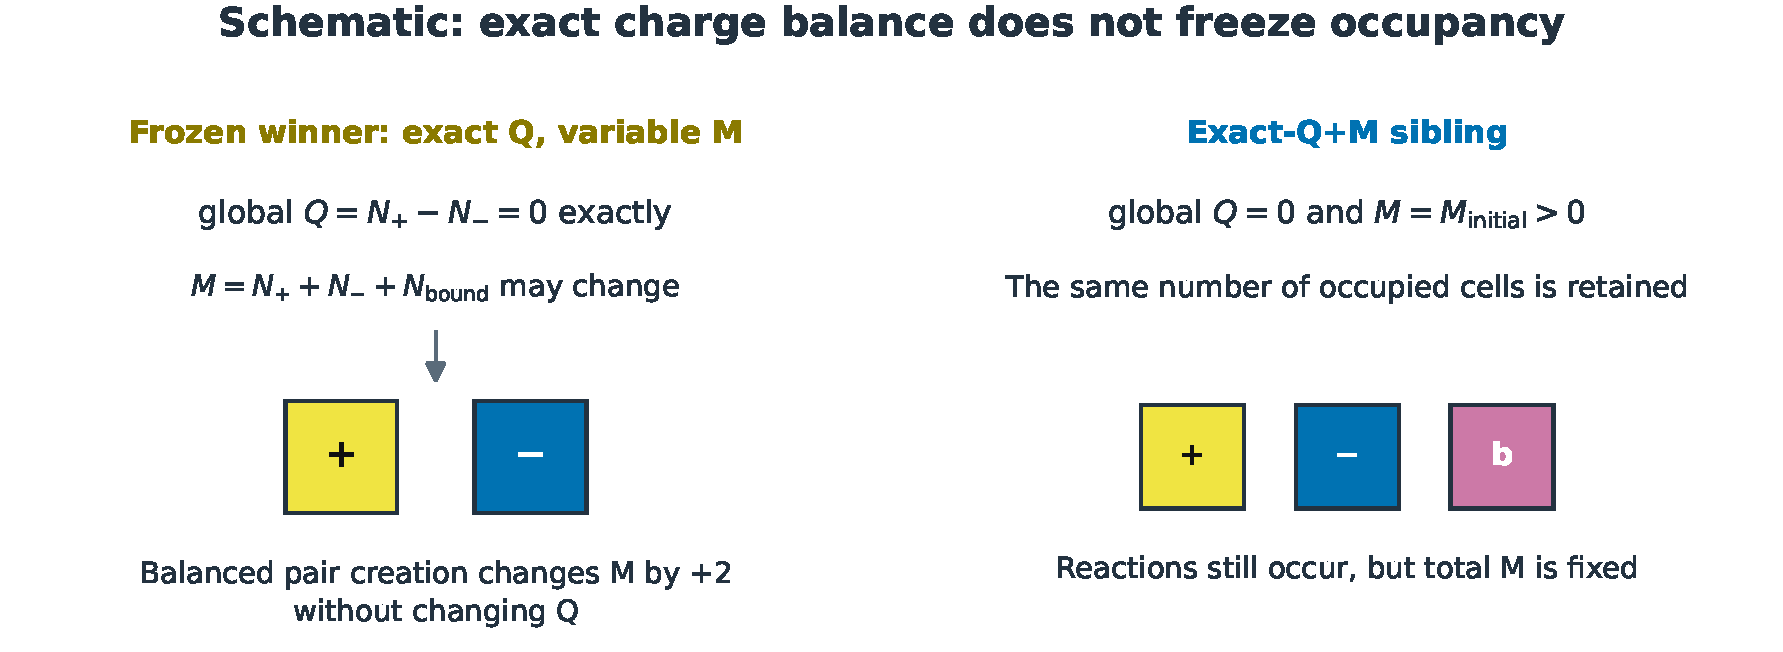
\includegraphics[scale=0.5]{FIGURE_07_MECHANISM_LEDGER_V135.pdf}
\caption{\textbf{Charge and occupancy.} Schematic: left, the winner conserves signed charge $Q$ while occupancy $M$ can change; right, the exact-$Q$+$M$ sibling conserves both, though its cells still react.}
\label{fig:ledger}
\end{figure}

\section{Discussion}
The experiments support a compact statement: a fully specified invertible block rule, restricted to the globally charge-balanced sector, can reorganise random material into very large irregular structures after widely spread, density-dependent waiting times, while remaining exactly reversible cell for cell. Crossing the endpoint is accompanied by substantial long-wave growth but high local compositional entropy. Distributed event morphology, an active exact-$Q{+}M$ sibling, transport-only controls, and reaction-pair ablations narrow the plausible mechanism without reducing it to a single reaction or established thermodynamic theory.

The closest precedents are substantive. Partitioned reversible automata supply the architecture \citep{Margolus1984,MoritaImai2001}; Q2R work supplies conservative reversible dynamics with macro-level relaxation \citep{UrbinaRica2016,Urbina2020}; reversible aggregation and reversible lattice gases demonstrate aggregation and apparent macroscopic irreversibility under invertible microscopic rules \citep{DSouzaMargolus1999,Broadwell2001}; one-dimensional two-species reversible automata supply especially close vacancy, species, reaction, and conserved-charge precedents \citep{MedenjakPopkovProsen2019,KlobasProsen2022}; and reactive lattice gases and reaction automata supply established pattern-forming contexts \citep{KapralLawniczakMasiar1991,BoonEtAl1996,WeimarBoon1994}. The residual contribution is the audited combination of a two-dimensional four-state signed invariant with variable occupancy, delayed distributed coarsening-like organisation, exact large-lattice reversal, and a frozen hierarchy of density, geometry, sibling, and reaction controls. The comparison rests on a bounded literature search, not a proof of exhaustive priority.

The broad waiting-time distribution invites comparison with rare-event and first-passage analysis \citep{BolhuisDellagoChandler1998,KaplanMeier1958}. Yet the data do not identify a free-energy barrier or stationary rate. Likewise, the separation between exact $Q$ and variable $M$ resembles theories coupling conserved and non-conserved fields, but only at a conceptual level \citep{HohenbergHalperin1977,Bray1994}. No equilibrium measure, temperature, or dynamic universality class has been demonstrated.

\needspace{10\baselineskip}
The coexistence of exact reversibility with directional-looking morphology also admits a precise qualification. Let $F$ be the complete finite update, partition phase included, and let $C$ be any onto map from complete states to a finite set of coarse descriptions. If the coarse description obeyed an exact autonomous law $f$ of its own, so that $CF=fC$ (which makes $C$ a factor map in the sense of symbolic dynamics \citep[Section~1.5]{LindMarcus1995}), then $f$ would have to be a permutation. Both $F$ and $C$ are onto, so $CF$ is onto, and therefore $f$ is onto; an onto map of a finite set to itself is invertible. This elementary observation rules out any account of the coarsening in which a fixed coarse description obeys an exact closed many-to-one macroscopic law; it says nothing against lossy descriptions, approximate coarse laws or history-dependent classifiers. It does not establish a thermodynamic arrow or identify a hidden causal precursor in these trajectories, and in particular it does not establish a history-erasure effect (Section~7): neither the recorded morphology nor the trajectory-prefix classifier is a demonstrated autonomous state description.

\section{Limitations and the shuffling test's failure}
\begin{corrbox}{The shuffling test and its endpoint}
The later v0.3.2 history-erasure campaign cannot support a causal reading. Global shuffling removed more than 99\% of the source's long-wave power. Yet the fixed endpoint classified many of the shuffled states as ``strong domain'' immediately or within a few thousand phases, because its connected-empty-cluster terms were confounded by the random high-occupancy geometry. In the primary cohort shuffled 32,768 phases before each source's own first hit (Branch B in the Supplement, 16 replicates), 9 hit at zero elapsed phases and 14 by 4,096 phases. The intervention audits and raw trajectories remain valid records, but the first-passage contrast is not a valid assay of preserved causal spatial memory. The experiment therefore does not show a necessary hidden multiscale precursor or a history-inhibition effect. Full diagnostics are in the Supplement.
\end{corrbox}

More generally, the study uses one selected winner, finite two-dimensional tori, finite horizons, operational morphology thresholds, and a bounded generator prevalence sample. Three readings that the vocabulary might invite are not supported by these finite-time data: that the density dependence is an equilibrium phase transition with a critical density; that the reversible yet directional-looking histories demonstrate a thermodynamic arrow; and that conserving $Q$ causes the organisation, rather than being a constraint under which it happens to occur.

For each fixed torus, the configuration together with the partition phase evolves by a permutation of a finite state space. Microscopic trajectories are therefore periodic, although their periods were not measured here; the reported coarsening-like behaviour is a finite-time macroscopic episode, not an asymptotic attracting phase.

\section{Reproducibility and evidence integrity}
The release records the raw unsigned-byte winner hash, exact configurations, seeds, horizons, endpoint definitions, compact CSV summaries, state hashes, figure-source hashes, code version, Windows/CUDA/PyTorch environment, and an independent parity audit. For that audit the frozen rule and the Margolus update were re-implemented in Eshkol, a Scheme-based language compiled to native code~\citep{Tsotchke2026Eshkol}: the generated program re-runs the exhaustive 256-entry audit (output range, one-to-one outputs, exact local charge) and replays a $16\times16$ exact-inventory torus for 256 phases (one partition phase per step), agreeing with the Python simulator cell for cell and in exact $Q$ and $M$. Full-resolution state arrays, checkpoints and complete trajectories are retained by the author and are not part of the public release; analyses that need them require the retained data or a new run. Figures are supplied in the formats listed in the release manifest, which records the size and SHA-256 digest of every included file. The release includes the intervention records and classifier diagnostics.

\section{Code and data availability}
A versioned archival deposit accompanies this paper, and a public repository carries a curated copy of it. The release includes the frozen rule tables and controls; forward and inverse simulation code; analysis and figure-generation code; tests and environment specifications; configurations, seeds and preregistration records; compact trajectory summaries and per-run results, including failures and censored runs; the endpoint diagnostics; and provenance records for the representative states shown in the figures. The state arrays themselves are retained by the author. These materials should support both independent scrutiny of the reported statistics and regeneration of the experiments without requiring all full-length trajectories to be stored in the repository.

\noindent\textbf{Archived code and data release:} Zenodo, DOI \href{https://doi.org/10.5281/zenodo.22270456}{\mbox{10.5281/zenodo.22270456}}.

\noindent\textbf{Public code repository:} \href{https://github.com/BartlettCJ/zws-reversible-coarsening}{github.com/BartlettCJ/zws-reversible-coarsening}, a curated copy of the release (code, evidence tables, paper sources and figures). The archived Zenodo release remains the citable, hash-pinned source for code, data and provenance.

The release manifest identifies the exact archived version, included files and any omitted large states or trajectories. Regeneration instructions distinguish what the compact release can reproduce directly from what requires a new simulation run.


\section{Conclusion}
In plain terms, this artificial world builds large, irregular structures out of random material without ever upsetting its overall plus--minus balance, and its microscopic evolution can be reversed cell for cell. The structures need not be crystals: the dense regions retain high local compositional disorder.

What matters is not the arithmetic of cancellation. It is that a simple, fully specified rule produces a reproducible pattern-forming regime, with long delays that depend strongly on starting occupancy and outcomes that change under targeted reaction controls. Fixing the net balance does not fix the amount of occupied material, its arrangement, or how those arrangements change. The active double-conservation sibling and the reaction-pair removals constrain this particular mechanism; they do not show that signed balance causes organisation or that changing occupancy is necessary in every reversible system.

The study therefore moves beyond a static example of quantities summing to zero to an experimentally characterised example of organised dynamics under that constraint.

\section*{Acknowledgements and AI-assistance statement}
Unlike the parent paper, \emph{Something is happening}, this companion paper is the product of a mostly autonomous AI research programme, and it is described as such deliberately. Chris Bartlett supplied the motivating idea, the parent paper's splitting-and-merging refinement conjecture, set the objective of testing it computationally, provided the hardware, and approved the scope and the stopping rules. He did not design the experiments, write the software, run the analyses, or draft the text. Those were done by AI systems: the experimental protocols, package releases and manuscript drafts by OpenAI's ChatGPT; the simulation campaigns and repository work by OpenAI Codex agents running unattended on the author's machine; and independent critical review by Anthropic's Claude models and by OpenAI's models. The author's part was to read the stage summaries, approve or redirect each next stage, commission the reviews, decide when to stop, and deposit the release; he accepts responsibility for the claims, interpretations and any remaining errors. Supporting project and review records are retained by the author. The independent parity oracle is written in Eshkol, a Scheme-based language by tsotchke released under the MIT licence~\citep{Tsotchke2026Eshkol}; its exhaustive rule audit and cell-for-cell replay are recorded in the release.

\bibliographystyle{unsrtnat}
\bibliography{references}

% Closing plate: a 512x512 window of the archived 1024x1024 state behind Figure 2, rendered cell for cell
% (provenance and hashes in figure_assets/plate_v025/plate_provenance.json).
\zwscolophon{figure_assets/plate_v025/plate_world_seed6203_phase311296_window512.png}{0.8\linewidth}{}{This world began as randomly scattered material, and at every step its plus and minus cells have cancelled to exactly zero. Yet it has sorted itself into large islands of busy material and empty channels: order at the large scale, made from a mixture that stays highly varied up close, and every step of that history could be run backwards exactly. A $512\times512$ window of the $1024\times1024$ world shown in Figure~\ref{fig:micro-macro} (initial occupancy 0.20, seed 6203, phase 311,296), rendered cell for cell from the archived state: yellow positive, blue negative, pink bound-neutral, black empty. Global $Q=0$; $M=431{,}677$ of 1,048,576 cells.}{Companion paper, version 1.49, 13 October 2026 $\cdot$ DOI 10.5281/zenodo.22270456}
\end{document}
